\documentclass{article}
\usepackage{graphicx} % Required for inserting images
\usepackage{biblatex}
\addbibresource{references.bib}
% \usepackage[sortcites=true,sorting=nyt,backend=biber]{biblatex}
\usepackage{hyperref}
\usepackage{amsmath}
\usepackage{amssymb}
\usepackage{caption}
\usepackage{subcaption}

\bibliography{references}

\title{Evolving Training Sets for Peptide Discrimination via Evolutionary Algorithms}
\author{Loek Gerrits (s1032343), Evangelos Spithas (s1125593), Bart van Nimwegen}
\date{\today}

\begin{document} 

\maketitle

\section{Introduction}

\subsection{Background}

In human bodies, the immune system is responsible for detecting pathogens and exterminating them. 
One of the tools at its disposal, is the T cells. T cells grow in the thymus, and each one is responsible for
identifying and attacking specific cells. However, that means that it is possible for healthy cells to be
attacked as well. In order to mitigate this, human cells are presented to the T cells, and the T cells that attack them 
are eliminated. This process is called Negative Selection (NS). In practice, the amount of possible cells is very large, and as a result only a sub-set of self peptides are presented
in the T cells. 

Artificial Immune Systems (AIS) are systems that draw inspiration from the human immune system, similarly to how Neural 
Networks (NNs) are inspired by the human nervous system. A big challenge in using the NS algorithm is selecting an effictive sub-set of peptides to train on.
Selecting the optimal subset is important because it direcly impacts the algorithm's ability to differentiate between healthy and harmful peptides.
Therefore being able to find the optimal subset to use for the NS algorithm is crucial to improve the accuracy of the NS algorithm.  

In this project, we would like to explore how we can find this optimal subsets to train an NS algorithm for peptide selection. We will do this using 3 different methods, randomly 
sampling a subset, using a greedy algorithm and an Evolutionary Algorithm (EA) to produce them. Afterwards, we will train the 
negative selection algorithm with each one of them, and evaluate its performance against different sets of harmful 
peptides, such as HIV and ebola cells. 

\subsection{Relevance}

\subsection{Problem description}

\subsection{Related work}


\cite{wortel2020t}


\section{Methodology}

\subsection{Optimizers} \label{optimizers}

In order to create more effective training dataset of self peptides for negative selection, we implemented two optimizers: 
1) a greedy algorithm and 2) the evolutionary algorithm. These strategies try to select subsets that maximize the information of the training data.



\subsubsection{Greedy Algorithm}

The greedy algorithm optimizes ...

Because the greedy algorithm has a high complexity, computing the fully optimized dataset using all human peptides and
all possible motifs was infeasible. Therefore, this study limited the number of peptides and motifs.


\subsubsection{Evolutionary Algorithm} 

\paragraph{AA composition}



\paragraph{AA frequency}

\paragraph{Exchangeability}







\subsection{Negative Selection}
In order to run the negative selection experiments we will use the jar that is provided by \url{https://johannes-textor.name/negativeselection.html}.
The training of the algorithm will take place with the three training sets as described in section \ref{datasets}.
All elements of each dataset have a fixed length of 6, and we will evaluate the effectiveness of the NS algorithm by 
experimenting  with a variable length of contiguous selectors, ranging between 1 and 6. 

For each peptide in the test datasets, the NS algorithm can return either the number of patterns in the repertoire that 
match it, or the normalised value $log_2(1 + x)$, where $x$ is the number of matching patterns. We will use this 
normalised value here, as the number of selectors can be unwieldy to work with. Afterwards, we can classify each peptide 
as anomalous or self peptide, if its score exceeds the value r.
% jar counts all matching selectors so we do log to get better anomaly scores

\subsection{Experimental design}
We set the following experimental setup to test our methods. We first generated three subsets of the english dataset 
from the text of Mobby Dick, with the methods described in section \ref{optimizers}, which we will use as the self set of 
the negative selection algorithm. The datasets have a size 3574. This was the size of the dataset returned by the greedy 
algorithm and was then used as the target size of the datasets of the other methods.

As test sets, we used an english dataset with 2000 english tokens, which were obtained by random excerpts from The Bible (\url{https://www.wordproject.org/bibles/index.htm}).
We also repeated the same method to obtain test datasets in the following languages: hiligaynon, latin, middle english, 
plautdietsch, tagalog and xhosa. The NS algorithm was run for each language, and after classifying the data, we 
estimated the receiver operating characteristic curve (AUC) to quantify how well our estimated datasets can optimise 
the NS algorithm.

Lastly, we repeated the same experiments but with actual peptide data. For that we used a subset of human peptides with 
size 126, as well peptides of the following diseases: HIV, hepatitis B, and ebola, as obtained by \url{https://github.com/ingewortel/negative-selection-2020}



\section{Results}
\subsection{Language Discrimination}
\begin{figure}[ht]
    \begin{subfigure}[t]{\linewidth}
        \centering
        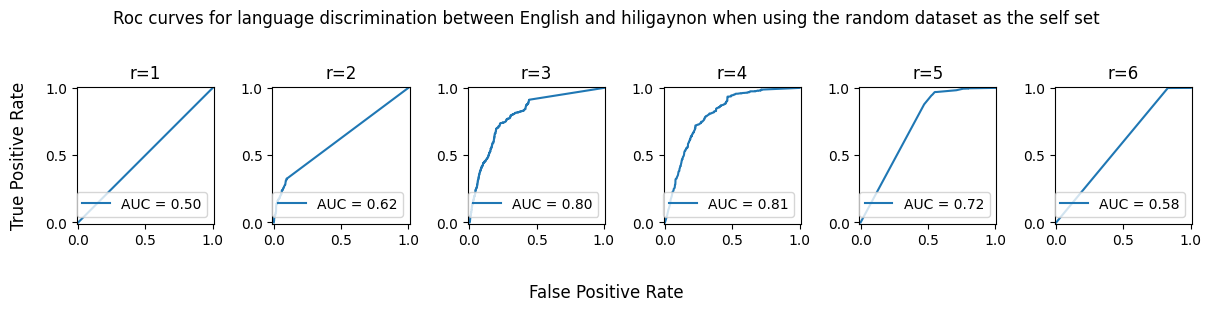
\includegraphics[width=\linewidth]{images/english_hiligayon_random.png}
        \label{fig:eng_hil_rnd}
    \end{subfigure}
    \\
    \begin{subfigure}[t]{\linewidth}
        \centering
        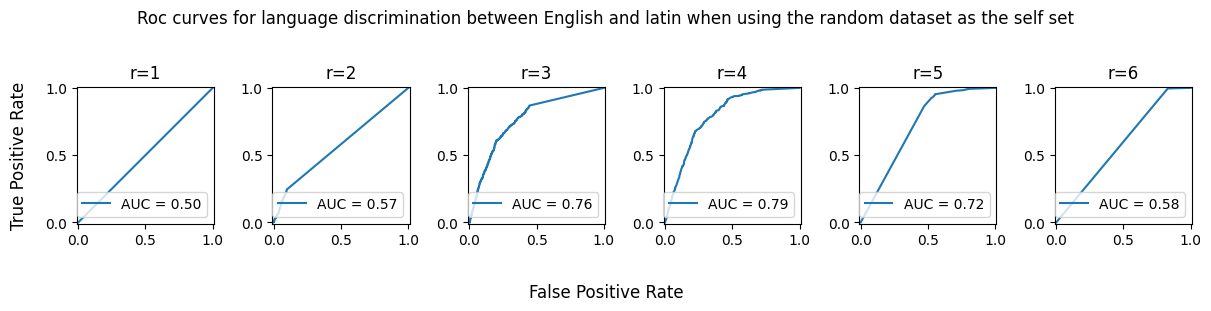
\includegraphics[width=\linewidth]{images/english_latin_random.png}
        \label{fig:eng_lat_rnd}
    \end{subfigure}
    \\
    \begin{subfigure}[t]{\linewidth}
        \centering
        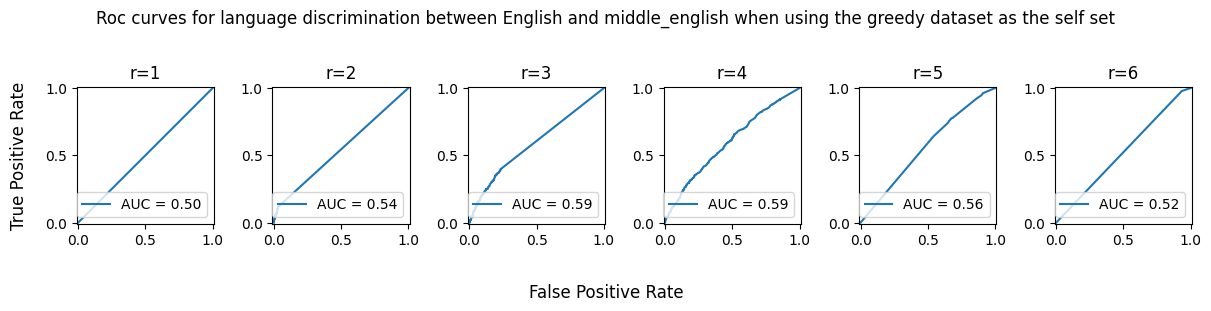
\includegraphics[width=\linewidth]{images/english_middle_neglish_greedy.png}
        \label{fig:eng_mid_eng_rnd}
    \end{subfigure}
    \\
    \begin{subfigure}[t]{\linewidth}
        \centering
        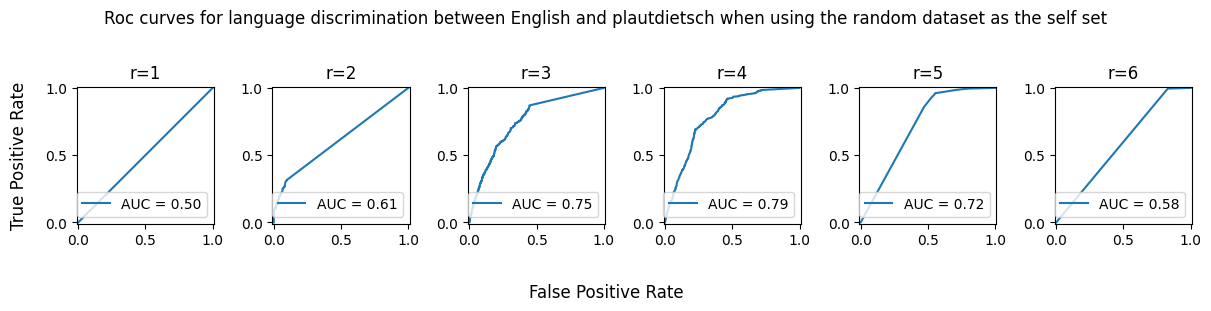
\includegraphics[width=\linewidth]{images/english_platudietsch_random.png}
        \label{fig:eng_mid_pla_rnd}
    \end{subfigure}
    \\
    \begin{subfigure}[t]{\linewidth}
        \centering
        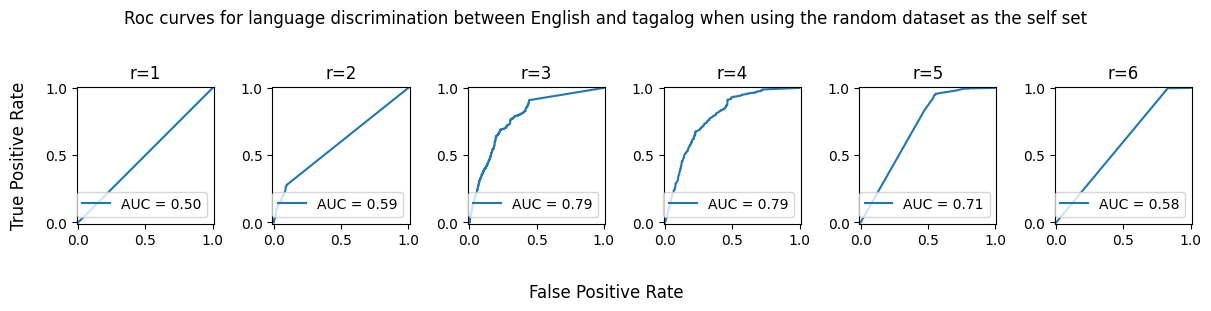
\includegraphics[width=\linewidth]{images/english_tagalog_random.png}
        \label{fig:eng_mid_tag_rnd}
    \end{subfigure}
        \\
    \begin{subfigure}[t]{\linewidth}
        \centering
        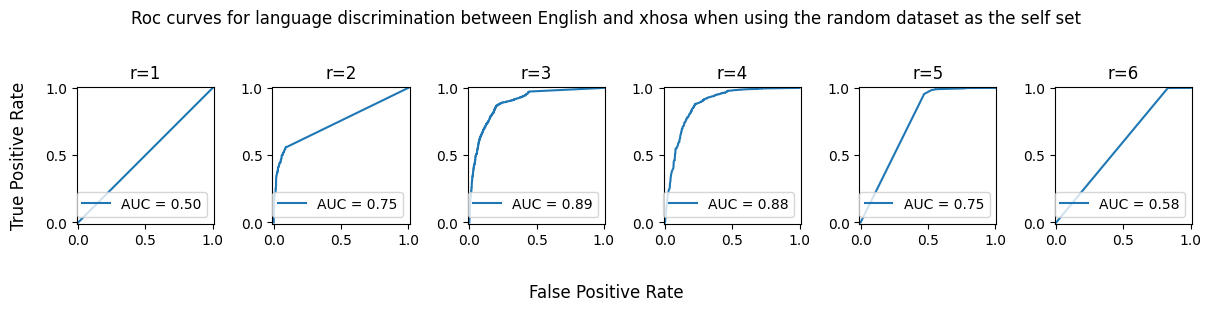
\includegraphics[width=\linewidth]{images/english_xhosa_random.png}
        \label{fig:eng_xho_rnd}
    \end{subfigure}\caption{ROC curves for language Discrimination between English and each other language, when using the random dataset for the self set}
\end{figure}
\subsection{Foreign Peptide Detection}



\section{Discussion}



\section{Conclusion}

The end.

\printbibliography

\appendix

\end{document}